\documentclass[]{article}
\usepackage[utf8]{inputenc}
\usepackage{polski}
\usepackage{listings}
\usepackage[usenames,dvipsnames]{xcolor}
\usepackage{geometry}
\usepackage{graphicx}
\usepackage{amsmath}
\usepackage{amssymb}
\usepackage{enumerate}
\DeclareGraphicsExtensions{.png}
\graphicspath{ {./} }
\geometry{
	a4paper,
	left=25mm,
	right = 25mm,
	top=25mm,
}
%%\hyphenchar\font=-1

\title{
	Sprawozdanie \\
	\large 
	Obliczenia naukowe - lista 2}
\author{Kamil Król}
\date{244949}


\begin{document}
	
	\maketitle
	
	\section*{Zadanie 1}
	Celem tego zadania było powtórzenie zadania 5 z listy 1, ale ze zmianą danych i zobaczenie jak te zmiany wpłynęły na wynik. Modyfikacja danych polegała na usunięciu ostatniej 9 z x4 i ostatniej 7 z x5. \newline
	Dane początkowe:\newline
	\mbox{$x_1$ = [2.718281828, -3.141592654, 1.414213562, 0.5772156649, 0.3010299957]}\newline
	\mbox{$y_1$ = [1486.2497, 878366.9879, -22.37492, 4773714.647, 0.000185049].}\newline
	Dane po modyfikacji:\newline
	\mbox{$x_2$ = [2.718281828, -3.141592654, 1.414213562, 0.577215664, 0.301029995]}\newline
	\mbox{$y_2$ = [1486.2497, 878366.9879, -22.37492, 4773714.647, 0.000185049].}\newline
	Poniżej wyniki dla obu zestawów.
	
	\begin{table}[h!]
		\centering
		\label{tab:table1}
		\begin{tabular}{|c|c|c|c|}
			\multicolumn{4}{c}{Dla Float64 dla danych $x_1$ i $y_1$}\\ \hline
			alogrytm & obliczona wartość & błąd bezwzględny & błąd względny\\
			\hline
			Forward & 1.0251881368296672e-10 & 1.1258452438296672e-10 & 11.184955313981627 \\ \hline
			Backward & -1.5643308870494366e-10 & 1.4636737800494365e-10 & 14.541186645165915 \\ \hline
			Descending & 0.0 & 1.00657107e-11 & 1.0 \\ \hline
			Ascending & 0.0 & 1.00657107e-11 & 1.0 \\ \hline
		\end{tabular}
	\end{table}

\begin{table}[h!]
	\centering
	\label{tab:table1}
	\begin{tabular}{|c|c|c|c|}
		\multicolumn{4}{c}{Dla Float64 dla danych $x_2$ i $y_2$}\\
		\hline
		alogrytm & obliczona wartość & błąd bezwzględny & błąd względny\\
		\hline
		Forward & -0.004296342739891585 & 4.526036594121319e-10 & 1.0534625357739803e-7 \\ \hline
		Backward & -0.004296342998713953 & 1.9378129136049527e-10 & 4.51037737625309e-8 \\ \hline
		Descending & -0.004296342842280865 & 3.502143800654389e-10 & 8.151452627834422e-8 \\ \hline
		Ascending & -0.004296342842280865 & 3.502143800654389e-10 & 8.151452627834422e-8 \\ \hline
	\end{tabular}
\end{table}


\begin{table}[h!]
	\centering
	\label{tab:table1}
	\begin{tabular}{|c|c|c|c|}
		\multicolumn{4}{c}{Dla Float32 dla danych $x_1$ i $y_1$}\\
		\hline
		alogrytm & obliczona wartość & błąd bezwzględny & błąd względny\\
		\hline
		Forward & -0.4999443 & 0.49994429944939167 & 4.9668057661282845e10 \\ \hline
		Backward & -0.4543457 & 0.4543457031149343 & 4.51379655800096e10 \\ \hline
		Descending & -0.5 & 0.4999999999899343 & 4.967359135306107e10 \\ \hline
		Ascending & -0.5 & 0.4999999999899343 & 4.967359135306107e10 \\ \hline
	\end{tabular}
\end{table}

\begin{table}[h!]
	\centering
	\label{tab:table1}
	\begin{tabular}{|c|c|c|c|}
		\multicolumn{4}{c}{Dla Float32 dla danych $x_2$ i $y_2$}\\
		\hline
		alogrytm & obliczona wartość & błąd bezwzględny & błąd względny\\
		\hline
Forward & -0.4999443 & 0.4956479562669622 & 115.36507538148926 \\ \hline
Backward & -0.4543457 & 0.4500493599325048 & 104.7517248432669 \\ \hline
Descending & -0.5 & 0.4957036568075048 & 115.37804002096217 \\ \hline
Ascending & -0.5 & 0.4957036568075048 & 115.37804002096217 \\ \hline
	\end{tabular}
\end{table}

Pierwszą obserwacją jest fakt, że wyniki dla typu Float32 są takie same dla obu zestawów testowych. Powodem takiego zachowania jest to, że wprowadzone zmiany nie zmieniły reprezentacji tych liczb w tej arytmetyce, ponieważ jej dokładność jest za mała. Drugą obserwacją jest to, że dla typu Float64 niewielkie zmiany w danych wejściowych spowodowały duże różnice w wynikach. W tej sytuacji usunięcie ostatnich cyfr zmniejszyło błąd reprezentacji dzięki czemu wyniki były dokładniejsze (widać to po znacznie mniejszych wartościach błędów względnych). Wnioskiem z zadania jest to, że obliczanie iloczynu skalarnego jest zadaniem źle uwarunkowanym.


	
	
	\section*{Zadanie 2}
	
	Celem zadania było narysowanie wykresu funkcji $f(x) = e^{x}\cdot ln(1+e^{-x})$ w dwóch dowolnych programach do wizualizacji. Ponadto należało obliczyć granicę funkcji \(\lim\limits_{x \to \infty}f(x)\) i porównać wynik z otrzymanymi wykresami. Zacząłem od obliczenia granicy: \(\lim\limits_{x \to \infty}f(x).\)
\begin{equation}
\begin{aligned}
\mathop {\lim }\limits_{x \to \infty} f(x) &= \mathop {\lim }\limits_{x \to \infty} e^x \ln(1 + e^{-x}) = \mathop {\lim }\limits_{x \to \infty} \dfrac{\ln(1 + e^{-x})}{e^{-x}} = \left[\dfrac{0}{0}\right] \stackrel{H}{=} \mathop {\lim }\limits_{x \to \infty} \dfrac{(\ln(1 + e^{-x}))'}{(e^{-x})'} = \\ 
&= \mathop {\lim }\limits_{x \to \infty} \dfrac{\frac{1}{1 + e^{-x}}\cdot -e^{-x}}{-e^{-x}} = \mathop {\lim }\limits_{x \to \infty} \dfrac{1}{1 + e^{-x}} = 1. \nonumber
\end{aligned}
\end{equation}
	
	 Poniżej wykresy z dwóch programów do wizualizacji.
	
	
	\begin{figure}[!htbp]
		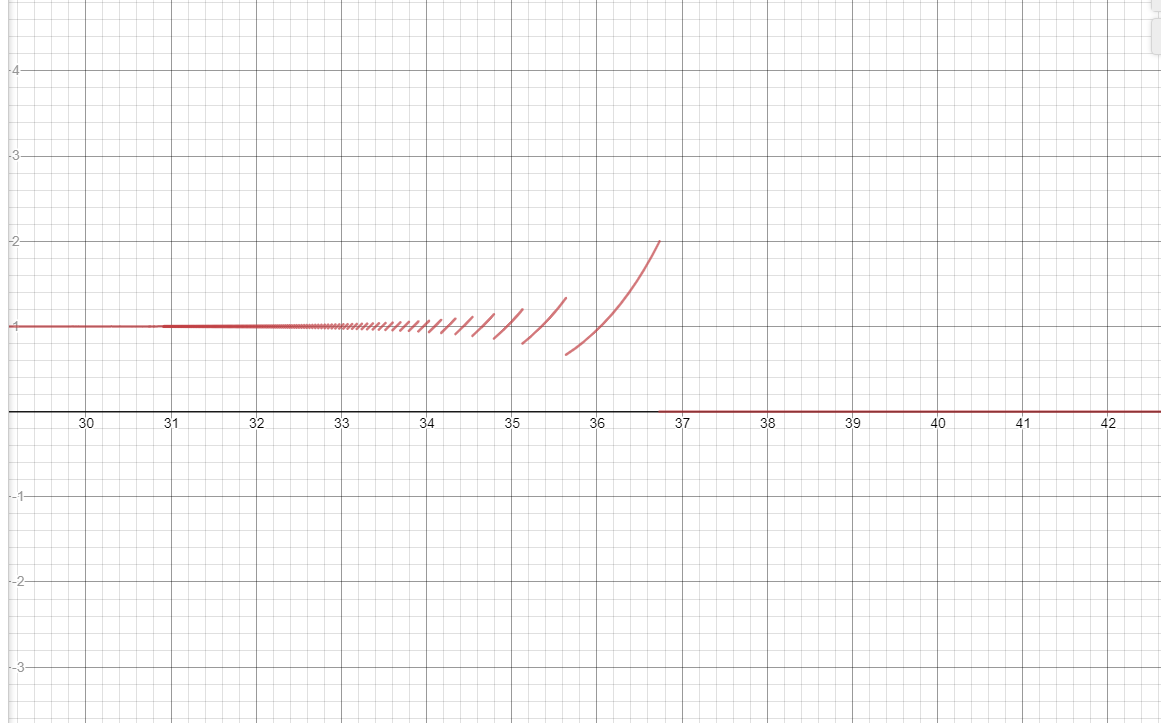
\includegraphics[scale=0.9]{task2_plot_desmos_broken}
		\centering
		\caption{Wykres funkcji f(x) narysowany w programie Desmos}
	\end{figure}
	\clearpage
	\begin{figure}[!htbp]
		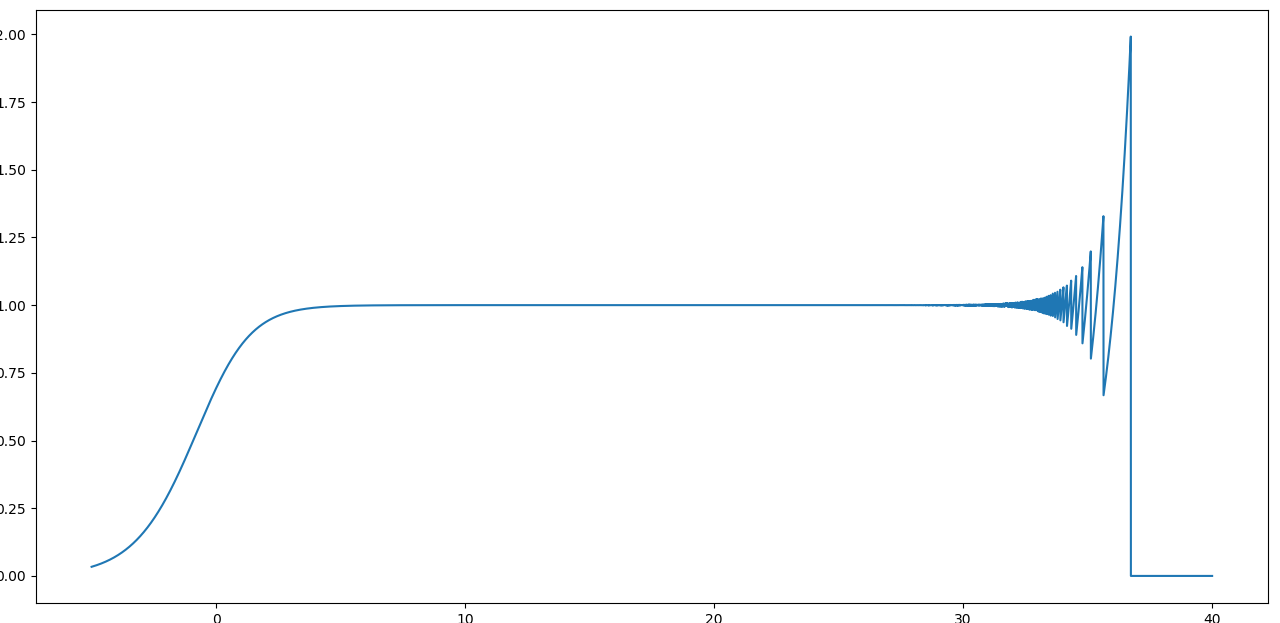
\includegraphics[scale=0.7]{task2_plot_pyplot}
		\centering
		\caption{Wykres funkcji f(x) narysowany w programie pyplot}
	\end{figure}

	Na wykresach można zaobserwować że dla x pomiędzy 30 a 40 funkcja zaczyna się zachowywać w nieoczekiwany sposób. Widać też, że dla dwóch programów zachowanie jest różne. Ponadto żaden z wykresów nie pokazuje właściwego przebiegu funkcji, ponieważ jej granicą przy x zmierzającym do nieskończoności jest 1, a nie jak sugerują wykresy wartość 0. Ostatnią rzeczą do zrobienia w tym zadaniu jest wyjaśnienie tego zjawiska. W tym celu przyjrzyjmy się dokładniej funkcji  $f(x) = e^{x}\cdot ln(1+e^{-x})$. Ze wzoru widać, że im większy argument x weźmiemy tym mamy do czynienia z mnożeniem coraz większej liczby z coraz mniejszą, a w związku z tym z utratą dokładności obliczeń. Jest to przyczyna oscylacji funkcji w przedziale $[30,40]$. Inna rzecz to \textit{to co dzieje się pod logarytmem}.
	Jest tam dodawanie liczby 1 do bardzo małej liczby (w przypadku odpowiednio dużego x). Jeżeli czynnik $e^{-x}$ jest odpowiednio mały to następuje zjawisko pochłonięcia tej wartości i otrzymujemy wartość 1.0. Zauważmy, że $e^{-37} < 2^{-53} < eps()$ oraz $ln(1) = 0$. Daje to w rezultacie mnożenie $e^{-x}\cdot ln(1)=e^{-x}\cdot0 = 0$, a następnie błędny wykres. Wnioskiem z zadania jest to, że bardzo małe zmiany w danych spowodowały duże różnice w wyniku. Zatem jest to przykład zadania, które jest źle uwarunkowane.
	
	\clearpage

	\section*{Zadanie 3} 
	
	Celem zadania jest wykonanie eksperymentów opisanych w treści zadania dotyczących rozwiązywania równania $\mathbf{Ax = b}$. Gdzie $\mathbf{A} \in \mathbb{R}^{n\times n}$,  $\mathbf{b} \in \mathbb{R}^n$.
	Macierz A zadana jest jako:
	\begin{enumerate}[a)]
		\item macierz Hilberta $\mathbf{H}_n$ stopnia $n$,
		\item macierz losowa $\mathbf{R}_n^c$ stopnia $n$ o danym wskaźniku uwarunkowania $c$.
	\end{enumerate}
	Wektor $\mathbf{b}$ dany jest jako $\mathbf{b = Ax}$, gdzie $\mathbf{x} = (1, \dots, 1)^{T}$. Dzięki temu znamy dokładne rozwiązanie dla A i b. Układ równań $\mathbf{Ax} = \mathbf{b}$ należało rozwiązać za pomocą dwóch algorytmów:
	\begin{enumerate}[a)]
		\item metodą eliminacji Gaussa: $\mathbf{x} = \mathbf{A} \backslash \mathbf{b}$,
		\item metodą macierzy odwrotnej: $\mathbf{x} = \mathbf{A}^{-1}\mathbf{b}$.
	\end{enumerate}
	Poniżej znajdują się wyniki eksperymentów.
	
	\begin{table}[h!]
		\centering
		\label{tab:table1}
		\begin{tabular}{|c|c|c|c|c|c|}
			\hline
			\multicolumn{5}{|c|}{Wyniki dla macierzy Hilberta} \\
			\hline
			rozmiar & rank & cond & błąd względny dla gaussa & błąd względny dla odwrotności \\ 
			\hline
			2 x 2 & 2 & 19.28147006790397 & 5.661048867003676e-16 & 1.4043333874306803e-15 \\ \hline
			3 x 3 & 3 & 524.0567775860644 & 8.022593772267726e-15 & 0.0 \\ \hline
			4 x 4 & 4 & 15513.73873892924 & 4.137409622430382e-14 & 0.0 \\ \hline
			5 x 5 & 5 & 476607.25024259434 & 1.6828426299227195e-12 & 3.3544360584359632e-12 \\ \hline
			6 x 6 & 6 & 1.4951058642254665e7 & 2.618913302311624e-10 & 2.0163759404347654e-10 \\ \hline
			7 x 7 & 7 & 4.75367356583129e8 & 1.2606867224171548e-8 & 4.713280397232037e-9 \\ \hline
			8 x 8 & 8 & 1.5257575538060041e10 & 6.124089555723088e-8 & 3.07748390309622e-7 \\ \hline
			9 x 9 & 9 & 4.931537564468762e11 & 3.8751634185032475e-6 & 4.541268303176643e-6 \\ \hline
			10 x 10 & 10 & 1.6024416992541715e13 & 8.67039023709691e-5 & 0.0002501493411824886 \\ \hline
			11 x 11 & 10 & 5.222677939280335e14 & 0.00015827808158590435 & 0.007618304284315809 \\ \hline
			12 x 12 & 11 & 1.7514731907091464e16 & 0.13396208372085344 & 0.258994120804705 \\ \hline
			13 x 13 & 11 & 3.344143497338461e18 & 0.11039701117868264 & 5.331275639426837 \\ \hline
			14 x 14 & 11 & 6.200786263161444e17 & 1.4554087127659643 & 8.71499275104814 \\ \hline
			15 x 15 & 12 & 3.674392953467974e17 & 4.696668350857427 & 7.344641453111494 \\ \hline
		\end{tabular}
	\end{table}

	\begin{table}[h!]
		\centering
		\label{tab:table1}
		\begin{tabular}{|c|c|c|c|c|c|}
			\hline
			\multicolumn{5}{|c|}{Wyniki dla macierzy losowej} \\
			\hline
			rozmiar & rank & cond & błąd względny dla gaussa & błąd względny dla odwrotności \\ 
			\hline
5 x 5 & 5 & $\approx1.0$ & 2.8522145930998397e-16 & 1.7901808365247238e-16 \\ \hline
5 x 5 & 5 & $\approx10.0$ & 6.861860919632454e-16 & 3.3674731643402955e-16 \\ \hline
5 x 5 & 5 & $\approx1000.0$ & 2.938162811804851e-14 & 2.585346872266395e-14 \\ \hline
5 x 5 & 5 & $\approx1.0e7$ & 1.600947789479836e-10 & 1.0757596219352109e-10 \\ \hline
5 x 5 & 5 & $\approx1.0e12$ & 1.7114279594016988e-5 & 2.257611195209549e-5 \\ \hline
5 x 5 & 4 & $\approx1.0e16$ & 0.23911323646084065 & 0.24987007579750867 \\ \hline
10 x 10 & 10 & $\approx1.0$ & 2.937374022976103e-16 & 2.579925170969555e-16 \\ \hline
10 x 10 & 10 & $\approx10.0$ & 3.040470972244059e-16 & 1.8242825833464351e-16 \\ \hline
10 x 10 & 10 & $\approx1000.0$ & 4.7589719986982775e-14 & 4.9583112156472015e-14 \\ \hline
10 x 10 & 10 & $\approx1.0e7$ & 5.908397149456726e-11 & 6.035098734232515e-11 \\ \hline
10 x 10 & 10 & $\approx1.0e12$ & 2.690988209513334e-5 & 2.8608639990839446e-5 \\ \hline
10 x 10 & 9 & $\approx1.0e16$ & 0.47733677715478207 & 0.44010801896736096 \\ \hline
20 x 20 & 20 & $\approx1.0$ & 5.4672143489065705e-16 & 3.5717446649531166e-16 \\ \hline
20 x 20 & 20 & $\approx10.0$ & 6.875319960193875e-16 & 7.182207712846219e-16 \\ \hline
20 x 20 & 20 & $\approx1000.0$ & 1.5382920267640914e-14 & 1.9531849215189054e-14 \\ \hline
20 x 20 & 20 & $\approx1.0e7$ & 4.936720925835152e-11 & 7.868469640811294e-11 \\ \hline
20 x 20 & 20 & $\approx1.0e12$ & 4.364457931127145e-6 & 3.844384073399806e-6 \\ \hline
20 x 20 & 19 & $\approx1.0e16$ & 0.015612189989446842 & 0.027926955723047063 \\ \hline
		\end{tabular}
	\end{table}

	Patrząc na tabelę pierwszą - wyniki dla macierzy Hilberta, można zauważyć zależność błędu względnego od wskaźnika uwarunkowania. Im większy jest wskaźnik uwarunkowania tym większy jest błąd. Macierz Hilberta jest przykładem macierzy, która jest bardzo źle uwarunkowana. Widać też, że metoda eliminacji Gaussa okazała się w tym przypadku dokładniejsza dla $n>7$. \newline
	Patrząc na tabelę drugą - wyniki dla macierzy losowej, można zauważyć taką samą zależność jak w eksperymencie pierwszym. Wartości błędów względnych są tym większe im więszke są wskaźniki uwarunkowania. Warto też zauważyć fakt, że dla dużej macierzy 20x20 o małym wskaźniku uwarunkowania np. c = 1, błąd względny jest znacznie mniejszy niż dla macierzy 5x5, która jest mniejsza, ale ma wskaźnik uwarunkowania równy $10^{16}$. Widać zatem, że wielkość macierzy nie jest tu czynnikiem decydującym. Najważniejszy jest wskaźnik uwarunkowania. Wnioskiem z zadania jest to, że wskaźnik uwarunkowania ma decydujący wpływ na dokładność obliczeń oraz to, że w przypadku obliczeń na macierzy źle uwarunkowanej należy się liczyć z dużymi błędami.
	
	\section*{Zadanie 4}

	Celem zadania było obliczenie dwudziestu zer wielomianu Wilkinsona w postaci naturalnej, a następnie sprawdzenie otrzymanych pierwiastków $z_k$ poprzez obliczenie $|P(z_k)|$, $|p(z_k)|$ i $|z_k-k|$ dla $1\leq k\leq 20$. Na końcu należało powtórzyć eksperyment Wilkinsona, który polegał na zamianie współczynnika przy $x^{19}$ równego $-210$ na $-210 -2^{23}$. Przez P będziemy oznaczać wielomian Wilkinsona w postaci naturalnej, a przez
	p ten sam wielomian w postaci iloczynowej.	
	$$p(x) = (x-20)(x-19)(x-18)\dots(x-6)(x-5)(x-4)(x-3)(x-2)(x-1)$$
	W poniższej tabeli znajdują się wyniki eksperymentu, który sprawdzał wartości pierwiastków.
	
	\begin{table}[h!]
		\centering
		\label{tab:table1}
		\begin{tabular}{|c|c|c|c|c|}
			\hline
			$k$ & $z_k$ & $|P(z_k)|$ & $|p(z_k)|$ & $|z_k-k|$ \\
			\hline
			1 & 0.9999999999996989 & 36352.0 & 5.517824e6 & 3.0109248427834245e-13 \\ \hline
			2 & 2.0000000000283182 & 181760.0 & 7.378697629901744e19 & 2.8318236644508943e-11 \\ \hline
			3 & 2.9999999995920965 & 209408.0 & 3.320413931687578e20 & 4.0790348876384996e-10 \\ \hline
			4 & 3.9999999837375317 & 3.106816e6 & 8.854437035384718e20 & 1.626246826091915e-8 \\ \hline
			5 & 5.000000665769791 & 2.4114688e7 & 1.8446752056545675e21 & 6.657697912970661e-7 \\ \hline
			6 & 5.999989245824773 & 1.20152064e8 & 3.320394888870126e21 & 1.0754175226779239e-5 \\ \hline
			7 & 7.000102002793008 & 4.80398336e8 & 5.423593016891272e21 & 0.00010200279300764947 \\ \hline
			8 & 7.999355829607762 & 1.682691072e9 & 8.26205014011023e21 & 0.0006441703922384079 \\ \hline
			9 & 9.002915294362053 & 4.465326592e9 & 1.196559421646318e22 & 0.002915294362052734 \\ \hline
			10 & 9.990413042481725 & 1.2707126784e10 & 1.6552601335207813e22 & 0.009586957518274986 \\ \hline
			11 & 11.025022932909318 & 3.5759895552e10 & 2.2478332979247994e22 & 0.025022932909317674 \\ \hline
			12 & 11.953283253846857 & 7.216771584e10 & 2.8869446884129956e22 & 0.04671674615314281 \\ \hline
			13 & 13.07431403244734 & 2.15723629056e11 & 3.807325552825022e22 & 0.07431403244734014 \\ \hline
			14 & 13.914755591802127 & 3.65383250944e11 & 4.612719853149547e22 & 0.08524440819787316 \\ \hline
			15 & 15.075493799699476 & 6.13987753472e11 & 5.901011420239329e22 & 0.07549379969947623 \\ \hline
			16 & 15.946286716607972 & 1.555027751936e12 & 7.01087410689741e22 & 0.05371328339202819 \\ \hline
			17 & 17.025427146237412 & 3.777623778304e12 & 8.568905825727875e22 & 0.025427146237412046 \\ \hline
			18 & 17.99092135271648 & 7.199554861056e12 & 1.0144799361089491e23 & 0.009078647283519814 \\ \hline
			19 & 19.00190981829944 & 1.0278376162816e13 & 1.1990376202486947e23 & 0.0019098182994383706 \\ \hline
			20 & 19.999809291236637 & 2.7462952745472e13 & 1.4019117414364248e23 & 0.00019070876336257925 \\ \hline
		\end{tabular}
	\end{table}

	Widać, że pierwiastki nie zostały obliczone dokładnie. Zwróćmy uwagę na wyniki dla k = 1, dla tego przypadku popełniony błąd bezwzględny był rzędu $10^{-13}$. Wydaje się, że nie jest to duży błąd. Kiedy popatrzymy na wartość wielomianu $|P(z_1)|$ to zamiast oczekiwanego 0, otrzymujemy 36352. Co dzieje się dla większych k? Dla k = 19 zamiast 0 otrzymujemy około $10^{13}$. Tak ogromny błąd całkowicie wyklucza sensowność obliczeń. 
	Kiedy popatrzymy na wartości $|p(z_k)|$ to popełnione błędy są jeszcze większe i sięgają rzędu $10^{23}$. Skąd wzięły się tak ogromne błędy? Na początku przyjrzyjmy się postaci normalnej wielomianu P. Ostatnie współczynniki P to między innymi: 13803759753640704000, -8752948036761600000 i 2432902008176640000. Jeżeli uwzględnimy fakt, że arytmetyka Float64 ma w języku Julia od 15 do 17 cyfr znaczących to widzimy, że współczynniki te nie dadzą się przechować dokładnie w tej arytmetyce. Stąd właśnie biorą się tak duże błędy przy obliczaniu $|P(z_k)|$. Teraz zobaczmy skąd biorą się błędy przy obliczaniu wartości $|p(z_k)|$. Zauważmy, że dla wielomianu w postaci iloczynowej błąd popełniony przy obliczaniu pierwiastka jest mnożony przez czynnik rzędu 19!. Stąd w tym przypadku biorą się tak ogromne błędy. 
	Teraz powtórzmy eksperyment Wilkinsona zamieniając w wielomianie P współczynnik -210 na $-210 -2^{23}$. W tabeli poniżej znajdują się pierwiastki zaburzonego wielomianu.
	
	\begin{table}[h!]
		\centering
		\label{tab:table1}
		\begin{tabular}{|c|c|}
			\hline
			część rzeczywista & część urojona \\
			\hline
			0.9999999999998357 & 0.0im \\ \hline
			2.0000000000550373 & 0.0im \\ \hline
			2.99999999660342 & 0.0im \\ \hline
			4.000000089724362 & 0.0im \\ \hline
			4.99999857388791 & 0.0im \\ \hline
			6.000020476673031 & 0.0im \\ \hline
			6.99960207042242 & 0.0im \\ \hline
			8.007772029099446 & 0.0im \\ \hline
			8.915816367932559 & 0.0im \\ \hline
			10.095455630535774 & -0.6449328236240688im \\ \hline
			10.095455630535774 & 0.6449328236240688im \\ \hline
			11.793890586174369 & -1.6524771364075785im \\ \hline
			11.793890586174369 & 1.6524771364075785im \\ \hline
			13.992406684487216 & -2.5188244257108443im \\ \hline
			13.992406684487216 & 2.5188244257108443im \\ \hline
			16.73074487979267 & -2.812624896721978im \\ \hline
			16.73074487979267 & 2.812624896721978im \\ \hline
			19.5024423688181 & -1.940331978642903im \\ \hline
			19.5024423688181 & 1.940331978642903im \\ \hline
			20.84691021519479 & 0.0im \\ \hline
		\end{tabular}
	\end{table}
	
	Widzimy, że zmiana jednego ze współczynników o wartość rzędu $2^{-23}$ sprawiła, że wielomian ma już pierwiastki zespolone. Wnioskiem z zadania jest fakt, że zadanie to jest źle uwarunkowane, ponieważ małe zaburzenia współczynników powodują znaczne zmiany w wynikach.
	
	\clearpage
	
	\section*{Zadanie 5}
	Celem zadania było wykonanie eksperymentów opisanych w treści zadania, które dotyczyły równania rekurencyjnego opisującego model logistyczny/model wzrostu populacji. Równanie:
	$$p_{n+1} := p_n + rp_n(1-p_n), \ \textrm{dla} \ n = 0, 1, \dots$$
	gdzie $r$ jest pewną daną stałą, $r(1-p_n)$ jest czynnikiem wzrostu populacji, a $p_0$ jest wielkością populacji stanowiącą procent maksymalnej wielkości populacji dla danego stanu środowiska.
	W tabeli poniżej znajdują się wyniki pierwszego eksperymentu polegającego na wykonaniu 40 iteracji danego wyrażenia rekurencyjnego w arytmetyce Float32 dla danych $p_0 = 0.01$ i $r = 3$, a później ponownym wykonananiu 40 iteracji, ale z obcięciem wyniku w iteracji 10.
	\begin{table}[!h]
		\centering
		\label{tab:table1}
		\begin{tabular}{|c|c|c|c|}
			\hline
			numer iteracji & bez modyfikacji & z modyfikacją \\
			\hline
			1 & 0.0397       & 0.0397 \\ \hline
			2 & 0.15407173   & 0.15407173 \\ \hline
			3 & 0.5450726    & 0.5450726 \\ \hline
			4 & 1.2889781    & 1.2889781 \\ \hline
			5 & 0.1715188    & 0.1715188 \\ \hline
			6 & 0.5978191    & 0.5978191 \\ \hline
			7 & 1.3191134    & 1.3191134 \\ \hline
			8 & 0.056273222  & 0.056273222 \\ \hline
			9 & 0.21559286   & 0.21559286 \\ \hline
			10 & 0.7229306    & 0.722 \\ \hline
			11 & 1.3238364    & 1.3241479 \\ \hline
			12 & 0.037716985  & 0.036488414 \\ \hline
			13 & 0.14660022   & 0.14195944 \\ \hline
			14 & 0.521926     & 0.50738037 \\ \hline
			15 & 1.2704837    & 1.2572169 \\ \hline
			16 & 0.2395482    & 0.28708452 \\ \hline
			17 & 0.7860428    & 0.9010855 \\ \hline
			18 & 1.2905813    & 1.1684768 \\ \hline
			19 & 0.16552472   & 0.577893 \\ \hline
			20 & 0.5799036    & 1.3096911 \\ \hline
			21 & 1.3107498    & 0.09289217 \\ \hline
			22 & 0.088804245  & 0.34568182 \\ \hline
			23 & 0.3315584    & 1.0242395 \\ \hline
			24 & 0.9964407    & 0.94975823 \\ \hline
			25 & 1.0070806    & 1.0929108 \\ \hline
			26 & 0.9856885    & 0.7882812 \\ \hline
			27 & 1.0280086    & 1.2889631 \\ \hline
			28 & 0.9416294    & 0.17157483 \\ \hline
			29 & 1.1065198    & 0.59798557 \\ \hline
			30 & 0.7529209    & 1.3191822 \\ \hline
			31 & 1.3110139    & 0.05600393 \\ \hline
			32 & 0.0877831    & 0.21460639 \\ \hline
			33 & 0.3280148    & 0.7202578 \\ \hline
			34 & 0.9892781    & 1.3247173 \\ \hline
			35 & 1.021099     & 0.034241438 \\ \hline
			36 & 0.95646656   & 0.13344833 \\ \hline
			37 & 1.0813814    & 0.48036796 \\ \hline
			38 & 0.81736827   & 1.2292118 \\ \hline
			39 & 1.2652004    & 0.3839622 \\ \hline
			40 & 0.25860548   & 1.093568 \\ \hline
		\end{tabular}
	\end{table}

	\clearpage

	W tabeli poniżej znajdują się wyniki eksperymentu drugiego, który polegał na wykonaniu 40 iteracji tego samego wyrażenia rekurencyjnego w arytmetyce Float32 oraz Float64 dla danych $p_0 = 0.01$ i $r = 3$, a później porównaniu otrzymanych wyników.

		\begin{table}[!h]
		\centering
		\label{tab:table1}
		\begin{tabular}{|c|c|c|c|}
			\hline
			numer iteracji & Float32 & Float64 \\
			\hline
			1 & 0.0397      	    &  0.0397 \\ \hline
			2 & 0.15407173  		& 0.15407173000000002 \\ \hline
			3 & 0.5450726   		& 0.5450726260444213 \\ \hline
			4 & 1.2889781   		& 1.2889780011888006 \\ \hline
			5 & 0.1715188   		& 0.17151914210917552 \\ \hline
			6 & 0.5978191   		& 0.5978201201070994 \\ \hline
			7 & 1.3191134   		& 1.3191137924137974 \\ \hline
			8 & 0.056273222 		& 0.056271577646256565 \\ \hline
			9 & 0.21559286  		& 0.21558683923263022 \\ \hline
			10 & 0.7229306  		& 0.722914301179573 \\ \hline
			11 & 1.3238364  		& 1.3238419441684408 \\ \hline
			12 & 0.037716985		& 0.03769529725473175 \\ \hline
			13 & 0.14660022 		& 0.14651838271355924 \\ \hline
			14 & 0.521926   		& 0.521670621435246 \\ \hline
			15 & 1.2704837  		& 1.2702617739350768 \\ \hline
			16 & 0.2395482  		& 0.24035217277824272 \\ \hline
			17 & 0.7860428  		& 0.7881011902353041 \\ \hline
			18 & 1.2905813  		& 1.2890943027903075 \\ \hline
			19 & 0.16552472 		& 0.17108484670194324 \\ \hline
			20 & 0.5799036  		& 0.5965293124946907 \\ \hline
			21 & 1.3107498  		& 1.3185755879825978 \\ \hline
			22 & 0.088804245		& 0.058377608259430724 \\ \hline
			23 & 0.3315584  		& 0.22328659759944824 \\ \hline
			24 & 0.9964407  		& 0.7435756763951792 \\ \hline
			25 & 1.0070806  		& 1.315588346001072 \\ \hline
			26 & 0.9856885  		& 0.07003529560277899 \\ \hline
			27 & 1.0280086  		& 0.26542635452061003 \\ \hline
			28 & 0.9416294  		& 0.8503519690601384 \\ \hline
			29 & 1.1065198  		& 1.2321124623871897 \\ \hline
			30 & 0.7529209  		& 0.37414648963928676 \\ \hline
			31 & 1.3110139  		& 1.0766291714289444 \\ \hline
			32 & 0.0877831  		& 0.8291255674004515 \\ \hline
			33 & 0.3280148  		& 1.2541546500504441 \\ \hline
			34 & 0.9892781  		& 0.29790694147232066 \\ \hline
			35 & 1.021099   		& 0.9253821285571046 \\ \hline
			36 & 0.95646656 		& 1.1325322626697856 \\ \hline
			37 & 1.0813814  		& 0.6822410727153098 \\ \hline
			38 & 0.81736827 		& 1.3326056469620293 \\ \hline
			39 & 1.2652004  		& 0.0029091569028512065 \\ \hline
			40 & 0.25860548 		& 0.011611238029748606 \\ \hline
		\end{tabular}
	\end{table}

	Z pierwszej tabeli widać, że zaburzenie wartości w 10 iteracji zmienia całkowicie wyniki w dalszych iteracjach. Od tego miejsca nie widać żadnej zależności między wynikami. Widać zatem, że w przypadku równania rekurencyjnego małe zaburzenie danych całkowicie zmieniło następne wyniki. Kolejna tabela pokazuje doświadczenie gdzie żadne zaburzenie nie zostało wprowadzone, jedyna różnica to arytmetyka w jakiej były wykonywane obliczenia. Widać, że na początku wartości są podobne, ale później tak jak w poprzednim eksperymencie zaczynają od siebie odbiegać dając na końcu zupełnie różne wyniki. Oba eksperymenty ukazują jak drobne błędy np. te związane z dokładnością przechowywanych danych mogą się kumulować i wpływać na wyniki. 
	Jest to zjawisko chaosu w układach sprzężeń zwrotnych. Czym są układy sprzężeń zwrotnych? Są to układy gdzie dane wyjściowe jednego procesu są danymi wejściowymi dla kolejnego kroku obliczeń. Wnioskiem z zadania jest to, że to równanie rekurencyjne jest niestabilne. Ponadto widać, że zjawisko chaosu jest trudne lub wręcz niemożliwe do wyeliminowania - dokładność obliczeń możemy ulepszyć poprzez zwiększanie precyzji arytmetyki, ale dla każdej arytmetyki pojawi się moment, w którym obliczenia stracą dokładność. 
	
	\section*{Zadanie 6}
	
	Celem zadania było sprawdzenie zachowania pewnego równania rekurencyjnego poprzez wykonanie 40 iteracji dla podanych w treści zadania zestawów danych. Równanie:
	$$x_{n+1} := x^2_n + c, \ \textrm{dla} \ n = 0,1,\dots$$
	
	Wyniki znajdują się w tabelach na końcu paragrafu.
	
	

	Obserwując wyniki dla c = -2 widać, że dla $x_0 = 1$ oraz dla $x_0 = 2$ rekurencja okazała się stabilna. Inna rzecz jaką można zauważyć, to fakt, że dla wartości nieznacznie odchylonej od 2.0 tzn. $x_0 = 1.99999999999999$ wyniki są zupełnie różne niż dla $x_0 = 2$. Widać zatem bardzo dużą czułość na warunki początkowe. Obserwując wyniki dla $c = -1$ widać, że otrzymane ciągi dla $x_0 = 1$ jak i $x_0 = -1$ są identyczne. Wynika to z podnoszenia tej wartości do kwadratu. Ostatnie dwie kolumny pokazują sytuację gdzie oba ciągi po jakimś czasie się stabilizują. Zarówno dla $x_0 = 0.25$ jak i $x_0 = 0.75$ otrzymujemy naprzemienne ciągi -1 i 1. Poniżej iteracje graficzne.
	

\begin{figure}[!htbp]
	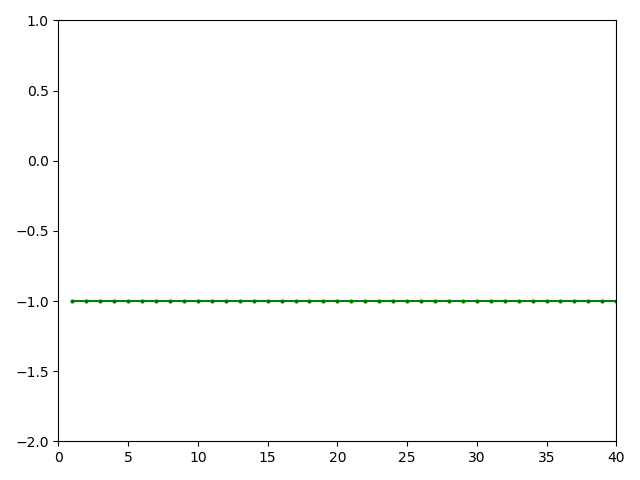
\includegraphics[scale=1]{task6-21}
	\centering
	\caption{$c = -2$, $x_0 = 1$}
\end{figure}
\clearpage
\begin{figure}[!htbp]
	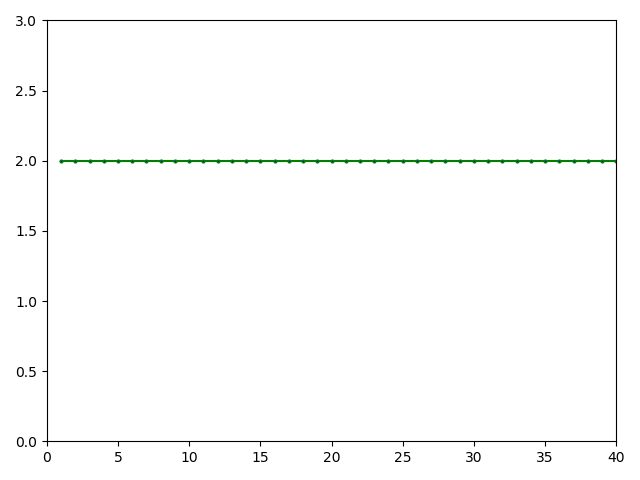
\includegraphics[scale=1]{task6-22}
	\centering
	\caption{$c = -2$, $x_0 = -1$}
\end{figure}
\begin{figure}[!htbp]
	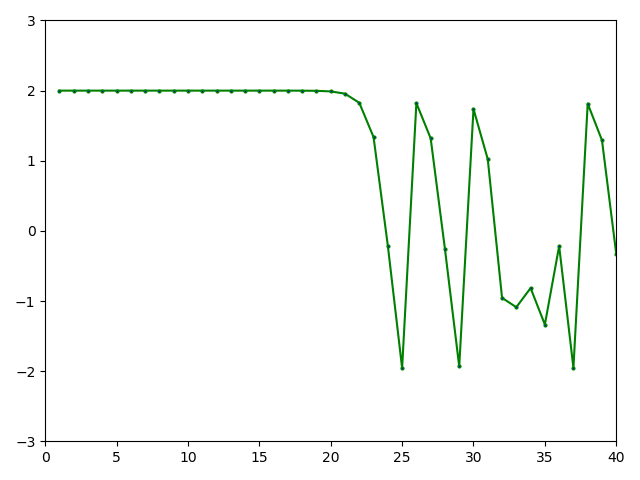
\includegraphics[scale=1]{task6-21,999.png}
	\centering
	\caption{$c = -2$, $x_0 = 1.99999999999999$}
\end{figure}
\begin{figure}[!htbp]
	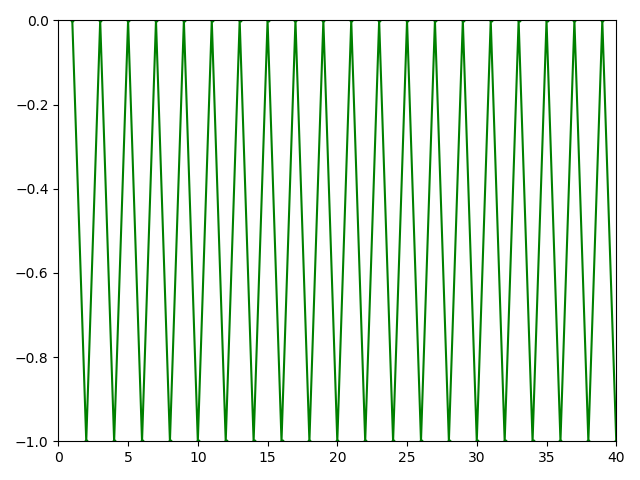
\includegraphics[scale=1]{task6-11}
	\centering
	\caption{$c = -1$, $x_0 = 1$}
\end{figure}
\begin{figure}[!htbp]
	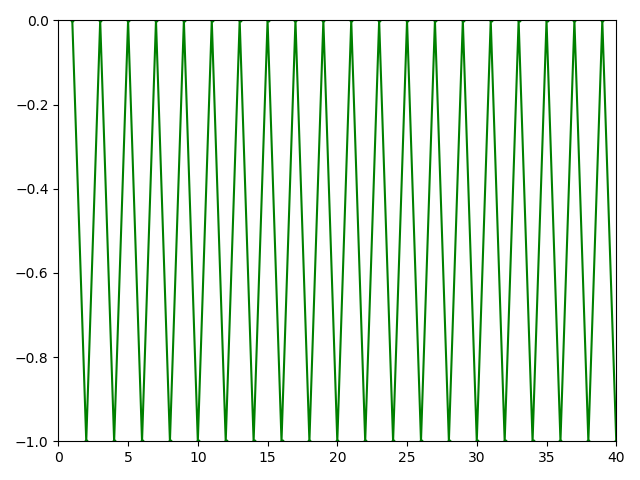
\includegraphics[scale=1]{task6-1-1}
	\centering
	\caption{$c = -1$, $x_0 = -1$}
\end{figure}
\begin{figure}[!htbp]
	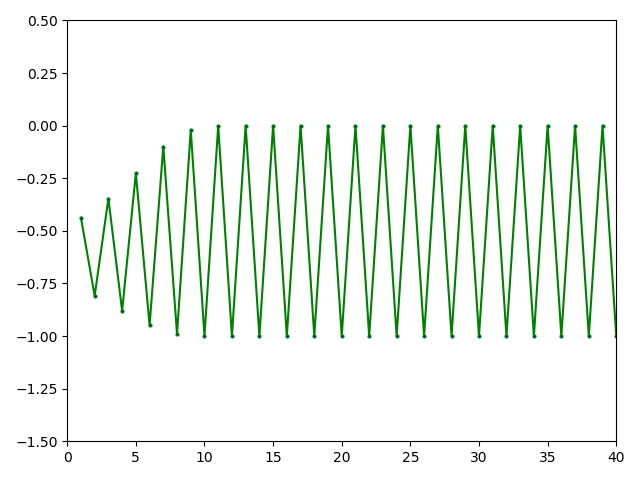
\includegraphics[scale=1]{task6-10,25}
	\centering
	\caption{$c = -1$, $x_0 = 0.25$}
\end{figure}
\begin{figure}[!htbp]
	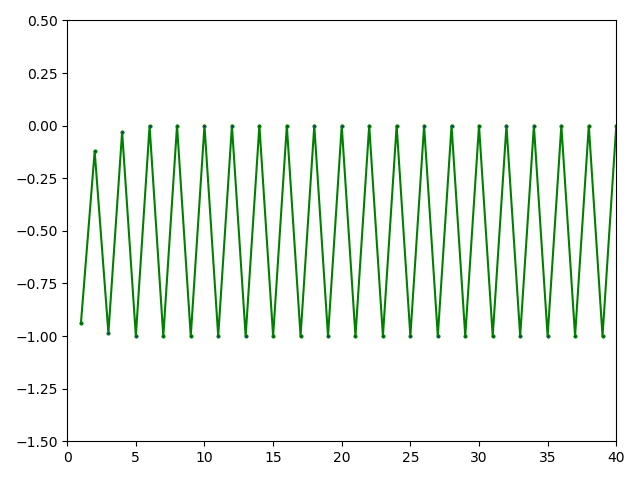
\includegraphics[scale=1]{task6-10,75}
	\centering
	\caption{$c = -1$, $x_0 = 0.75$}
\end{figure}


Wnioski. Zauważmy, że w tym zadaniu również mamy do czynienia ze zjawiskiem sprzężenia zwrotnego. W całym zadaniu możemy wyróżnić 3 typy doświadczeń. Pierwszy z nich to dwa pierwsze doświadczenia oraz te z c = -1 i $x_0 \in \{-1,1\}$, w którch otrzymano ciągi stałe lub naprzemienne, są to układy stabilne. Drugi typ to doświadczenie z $x_0 = 1.99999999999999$. Tutaj ciąg był chaotyczny. Jest to układ niestabilny. Trzeci typ doświadczenia reprezentują dwa ostatnie eksperymenty. W obu z nich układ początkowo był chaotyczny, ale po którymś kroku zaczął się stabilizować. Są to układy stabilne.

	
	\begin{table}[!h]
		\centering
		\label{tab:table1}
		\begin{tabular}{|c|c|c|c|}
			\multicolumn{4}{c}{$c = -2$} \\
			\hline
			numer iteracji & $x_0 = 1$ & $x_0 = 2$ & $x_0 = 1.99999999999999$\\
			\hline
			1 & -1 &	 2 &	 1.99999999999996 \\ \hline
			2 & -1 &	 2 &	 1.9999999999998401 \\ \hline
			3 & -1 &	 2 &	 1.9999999999993605 \\ \hline
			4 & -1 &	 2 &	 1.999999999997442 \\ \hline
			5 & -1 &	 2 &	 1.9999999999897682 \\ \hline
			6 & -1 &	 2 &	 1.9999999999590727 \\ \hline
			7 & -1 &	 2 &	 1.999999999836291 \\ \hline
			8 & -1 &	 2 &	 1.9999999993451638 \\ \hline
			9 & -1 &	 2 &	 1.9999999973806553 \\ \hline
			10 & -1 &	 2 &	 1.999999989522621 \\ \hline
			11 & -1 &	 2 &	 1.9999999580904841 \\ \hline
			12 & -1 &	 2 &	 1.9999998323619383 \\ \hline
			13 & -1 &	 2 &	 1.9999993294477814 \\ \hline
			14 & -1 &	 2 &	 1.9999973177915749 \\ \hline
			15 & -1 &	 2 &	 1.9999892711734937 \\ \hline
			16 & -1 &	 2 &	 1.9999570848090826 \\ \hline
			17 & -1 &	 2 &	 1.999828341078044 \\ \hline
			18 & -1 &	 2 &	 1.9993133937789613 \\ \hline
			19 & -1 &	 2 &	 1.9972540465439481 \\ \hline
			20 & -1 &	 2 &	 1.9890237264361752 \\ \hline
			21 & -1 &	 2 &	 1.9562153843260486 \\ \hline
			22 & -1 &	 2 &	 1.82677862987391 \\ \hline
			23 & -1 &	 2 &	 1.3371201625639997 \\ \hline
			24 & -1 &	 2 &	 -0.21210967086482313 \\ \hline
			25 & -1 &	 2 &	 -1.9550094875256163 \\ \hline
			26 & -1 &	 2 &	 1.822062096315173 \\ \hline
			27 & -1 &	 2 &	 1.319910282828443 \\ \hline
			28 & -1 &	 2 &	 -0.2578368452837396 \\ \hline
			29 & -1 &	 2 &	 -1.9335201612141288 \\ \hline
			30 & -1 &	 2 &	 1.7385002138215109 \\ \hline
			31 & -1 &	 2 &	 1.0223829934574389 \\ \hline
			32 & -1 &	 2 &	 -0.9547330146890065 \\ \hline
			33 & -1 &	 2 &	 -1.0884848706628412 \\ \hline
			34 & -1 &	 2 &	 -0.8152006863380978 \\ \hline
			35 & -1 &	 2 &	 -1.3354478409938944 \\ \hline
			36 & -1 &	 2 &	 -0.21657906398474625 \\ \hline
			37 & -1 &	 2 &	 -1.953093509043491 \\ \hline
			38 & -1 &	 2 &	 1.8145742550678174 \\ \hline
			39 & -1 &	 2 &	 1.2926797271549244 \\ \hline
			40 & -1 &	 2 &	 -0.3289791230026702 \\ \hline
		\end{tabular}
	\end{table}
	
	\begin{table}[!h]
		\centering
		\label{tab:table1}
		\begin{tabular}{|c|c|c|c|c|}
			\multicolumn{5}{c}{$c = -1$} \\
			\hline
			numer iteracji & $x_0 = 1$ & $x_0 = -1$ & $x_0 = 0.25$ & $x_0 = 0.75$ \\
			\hline
			1	&0 &	0 &	-0.4375 &	 -0.9375 \\ \hline	
			2	& -1 &	 -1 &	 -0.80859375 &	 -0.12109375 \\ \hline	
			3	& 0 &	 0 &	 -0.3461761474609375 &	 -0.9853363037109375 \\ \hline	
			4	& -1 &	 -1 &	 -0.8801620749291033 &	 -0.029112368589267135 \\ \hline	
			5	& 0 &	 0 &	 -0.2253147218564956 &	 -0.9991524699951226 \\ \hline	
			6	& -1 &	 -1 &	 -0.9492332761147301 &	 -0.0016943417026455965 \\ \hline	
			7	& 0 &	 0 &	 -0.0989561875164966 &	 -0.9999971292061947 \\ \hline	
			8	& -1 &	 -1 &	 -0.9902076729521999 &	 -5.741579369278327e-6 \\ \hline	
			9	& 0 &	 0 &	 -0.01948876442658909 &	 -0.9999999999670343 \\ \hline	
			10&	 -1 &	 -1 &	 -0.999620188061125 &	 -6.593148249578462e-11 \\ \hline	
			11&	 0 &	 0 &	 -0.0007594796206411569 &	 -1.0 \\ \hline	
			12&	 -1 &	 -1 &	 -0.9999994231907058 &	 0.0 \\ \hline	
			13&	 0 &	 0 &	 -1.1536182557003727e-6 &	 -1.0 \\ \hline	
			14&	 -1 &	 -1 &	 -0.9999999999986692 &	 0.0 \\ \hline	
			15&	 0 &	 0 &	 -2.6616486792363503e-12 &	 -1.0 \\ \hline	
			16&	 -1 &	 -1 &	 -1.0 &	 0.0 \\ \hline	
			17&	 0 &	 0 &	 0.0 &	 -1.0 \\ \hline	
			18&	 -1 &	 -1 &	 -1.0 &	 0.0 \\ \hline	
			19&	 0 &	 0 &	 0.0 &	 -1.0 \\ \hline	
			20&	 -1 &	 -1 &	 -1.0 &	 0.0 \\ \hline	
			21&	 0 &	 0 &	 0.0 &	 -1.0 \\ \hline	
			22&	 -1 &	 -1 &	 -1.0 &	 0.0 \\ \hline	
			23&	 0 &	 0 &	 0.0 &	 -1.0 \\ \hline	
			24&	 -1 &	 -1 &	 -1.0 &	 0.0 \\ \hline	
			25&	 0 &	 0 &	 0.0 &	 -1.0 \\ \hline	
			26&	 -1 &	 -1 &	 -1.0 &	 0.0 \\ \hline	
			27&	 0 &	 0 &	 0.0 &	 -1.0 \\ \hline	
			28&	 -1 &	 -1 &	 -1.0 &	 0.0 \\ \hline	
			29&	 0 &	 0 &	 0.0 &	 -1.0 \\ \hline	
			30&	 -1 &	 -1 &	 -1.0 &	 0.0 \\ \hline	
			31&	 0 &	 0 &	 0.0 &	 -1.0 \\ \hline	
			32&	 -1 &	 -1 &	 -1.0 &	 0.0 \\ \hline	
			33&	 0 &	 0 &	 0.0 &	 -1.0 \\ \hline	
			34&	 -1 &	 -1 &	 -1.0 &	 0.0 \\ \hline	
			35&	 0 &	 0 &	 0.0 &	 -1.0 \\ \hline	
			36&	 -1 &	 -1 &	 -1.0 &	 0.0 \\ \hline	
			37&	 0 &	 0 &	 0.0 &	 -1.0 \\ \hline	
			38&	 -1 &	 -1 &	 -1.0 &	 0.0 \\ \hline	
			39&	 0 &	 0 &	 0.0 &	 -1.0 \\ \hline	
			40&	 -1 &	 -1 &	 -1.0 &	 0.0 \\ \hline	
		\end{tabular}
	\end{table}


\end{document}